\documentclass{rbfin}
\usepackage{amsmath}
\usepackage{amssymb} %mathbb
\usepackage{gensymb} % \degree
\usepackage{graphicx}
\usepackage{hyperref}

\begin{document}
\selectlanguage{brazil}
\shorttitle{Otimização Não Linear 2021} % appears on header every other page
\rbfe{}
\autor{Vinícius Claudino Ferraz, 2021}

\begin{center}
\Large

\textbf{Lista 3}

\normalsize

Matrícula $= 2019435823$
\end{center}

\large

\textbf{Questão 1.A}

\normalsize

\vspace{6mm}

\doublespacing

Ache o mínimo da função $f(x) = 0.65 - \cfrac{0.75}{1 + x^2} - 0.65 x \arctan \cfrac{1}{x}$ utilizando busca irrestrita com um tamanho de passo fixo de $0.1$ partindo do ponto $0.0$.

Pelo método do gráfico (questão $2$), o mínimo exato ocorre em $x^* = 0.4804805$, $f(x^*) = -0.3100204$.

Para $x_0 = 0$ ; $\delta = 0.1$ ; $x_i = x_0 + i\delta$ ;

$f(x_0) > f(x_1) > f(x_2) > f(x_3) > f(x_4) > f(x_5) < f(x_6)$.

$-0.1 > -0.1881976 > -0.2496959 > -0.2875446 > -0.3060271 > -0.3098233 < -0.3033175$.

Portanto, o mínimo ocorre em $x^* = 0.5$, $f(x^*) = -0.3098233$. A acurácia é $1 - \cfrac{0.3098233}{0.3100204} = 0.06356573\%$.

\singlespacing

\vspace{6mm}

\large

\textbf{Questão 1.B}

\normalsize

\vspace{6mm}

\doublespacing

Ache o mínimo da função $f(x)$ utilizando busca irrestrita com um tamanho de passo acelerado iniciando com um tamanho de $0.1$ partindo do ponto $0.0$.

Para $x_0 = 0$ ; $x_1 = 0.1$ ; $x_2 = 0.2$ ; $x_3 = 0.4$ ; $x_4 = 0.8$ ;

$f(x_0) > f(x_1) > f(x_2) > f(x_3) < f(x_4)$.

$-0.1 > -0.1881976 > -0.2496959 > -0.3060271 < -0.27326587$.

Portanto, o mínimo ocorre em $x^* = 0.4$, $f(x^*) = -0.3060271$. A acurácia é $1 - \cfrac{0.3060271}{0.3100204} = 1.288073\%$.

\singlespacing

\vspace{6mm}

\large

\textbf{Questão 1.C}

\normalsize

\vspace{6mm}

\doublespacing

Ache o mínimo da função $f(x)$ utilizando busca exaustiva no intervalo $(0, 3)$ até atingir uma acurácia de $5\%$ do valor exato.

Dividimos em $n = 4$ pontos interiores: $v = (0.0, 0.6, 1.2, 1.8, 2.4, 3.0)$.

Calculamos $f$ em cada coordenada: $fv = (-0.1, -0.30331755, -0.19927290, -0.12019204, -0.07682089, -0.05241358)$.

A acurácia da segunda coordenada é $1 - \cfrac{0.30331755}{0.3100204} = 2.162067\%$.

Portanto, o mínimo ocorre em $x^* = 0.6$, $f(x^*) = -0.30331755$.

\singlespacing

\newpage

\large

\textbf{Questão 1.D}

\normalsize

\vspace{6mm}

\doublespacing

Ache o mínimo da função $f(x)$ utilizando busca dicotômica no intervalo $(0, 3)$ até obter uma acurácia de $5\%$ do valor exato, com um $\delta = 0.0001$.

Inserimos $2$ pontos interiores: $v_1 = (0.0, 1.49995, 1.50005, 3.0)$.

Calculamos $f$ em cada coordenada: $fv_1 = (-0.1, -0.1540783, -0.1540652, -0.05241358)$.

O novo intervalo é $[0, 1.50005]$. Inserimos $2$ pontos interiores: $v_2 = (0, 0.749975, 0.750075, 1.50005)$.

Calculamos $f$ em cada coordenada: $fv_2 = (-0.1, -0.1540783, -0.1540652, -0.05241358)$.

O novo intervalo é $[0, 0.750075]$. No ponto médio, $f(0.3750375) = -0.3029708$.

A acurácia é $1 - \cfrac{0.3029708}{0.3100204} = 2.27391\%$.

Portanto, o mínimo ocorre em $x^* = 0.3750375$, $f(x^*) = -0.3029708$.

\singlespacing

\vspace{6mm}

\large

\textbf{Questão 1.E}

\normalsize

\vspace{6mm}

\doublespacing

Ache o mínimo da função $f(x)$ utilizando busca da bisseção no intervalo $(0, 3)$ até obter uma acurácia de $5\%$ do valor exato.

Inserimos $3$ pontos interiores: $v_1 = (x_1 = 0.75, x_0 = 1.50, x_2 = 2.25)$.

Calculamos $f$ em cada coordenada: $fv_1 = (-0.28205642, -0.15407177, -0.08536442)$. Mínimo $= x_1$.  

O novo intervalo é $[0, 1.50]$. Inserimos $3$ pontos interiores: $v_2 = (x_1 = 0.375, x_0 = 0.750, x_2 = 1.125)$.

Calculamos $f$ em cada coordenada: $fv_2 = (-0.3029655, -0.2820564, -0.2123917)$. Mínimo $= x_1$.

O novo intervalo é $[0, 0.75]$. No ponto médio, $f(0.375) = -0.3029655$.

A acurácia é $1 - \cfrac{0.3029655}{0.3100204} = 2.275624\%$.

Portanto, o mínimo ocorre em $x^* = 0.375$, $f(x^*) = -0.3029655$.

\singlespacing

\vspace{6mm}

\large

\textbf{Questão 2} 

\normalsize

\vspace{6mm}

\doublespacing

Faça o gráfico da função $f(x)$ no intervalo $(0, 3)$ e identifique o mínimo.

\begin{center}
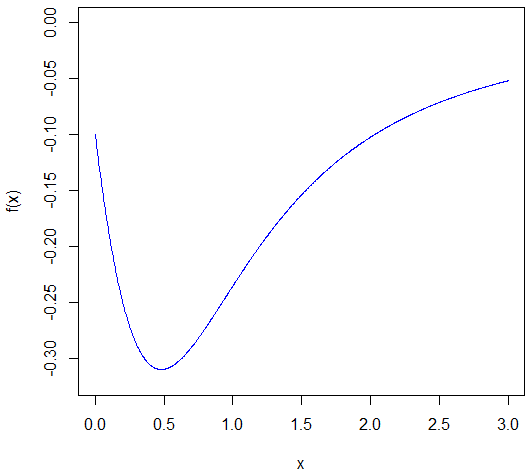
\includegraphics[scale=0.666]{q2}
\end{center}

O mínimo ocorre em $x^* = 0.4804805$, $f(x^*) = -0.3100204$. Fontes abaixo:

\singlespacing

\begin{verbatim}
f <- function(x) {
   return (0.65 - 0.75/(1 + x^2) - 0.65 * x * atan(1/x))
}
   
dev.off()
Mx1 <- 0
Mx2 <- 3
My1 <- -0.32
My2 <- 0
N <- 1000
x <- matrix(0, N)
y <- matrix(0, N)
for (i in 1:N) {
   # t(1) = Mx1, t(N) = Mx2
   t <- (Mx2 - Mx1)/(N - 1) * (i - 1) + Mx1 
   x[i] <- t
   y[i] <- f(t)
}
plot(x,y,type = 'l',col='blue',xlim=c(Mx1,Mx2),ylim = c(My1,My2),xlab='x',ylab='f(x)')
min(y)
for (i in 1:N)
   if (y[i] == min(y))
      print(x[i])
\end{verbatim}

\vspace{6mm}

\large

\textbf{Questão 3.A}

\normalsize

\vspace{6mm}

\doublespacing

Ache o máximo da função $g(x) = \cfrac{0.5}{\sqrt{1 + x^2}} - \sqrt{1 + x^2} \left( 1 - \cfrac{0.5}{1 + x^2} \right) + x$ utilizando busca irrestrita com um tamanho de passo fixo de $0.1$ partindo do ponto $0.0$.

Pelo método do gráfico (questão $2$), o máximo exato ocorre em $x^* = 0.7867868$, $g(x^*) = 0.300283$.

Para $x_0 = 0$ ; $\delta = 0.1$ ; $x_i = x_0 + i\delta$ ;

$g(x_0) < g(x_1) < g(x_2) < g(x_3) < g(x_4) < g(x_5) < g(x_6) < g(x_7) < g(x_8) > g(x_9)$.

$0 < 0.09004963 < 0.1607768 < 0.2137956 < 0.2514437 < 0.2763932 < 0.2913025 < 0.2985764 < 0.300244 >$

$> 0.2979317$.

Portanto, o máximo ocorre em $x^* = 0.8$, $g(x^*) = 0.300244$. A acurácia é $1 - \cfrac{0.300244}{0.300283} = 0.01300042\%$.

\singlespacing

\begin{verbatim}
#busca irrestrita, passo fixo

f <- function(x) {
   #return (0.65 - 0.75/(1 + x^2) - 0.65 * x * atan(1/x))
   return (-0.5/sqrt(1 + x^2) + sqrt(1 + x^2) * ( 1 - 0.5/(1 + x^2) ) - x)
}

exato <- -0.300283 # -0.3100204 
x0 <- 0
delta <- 0.1
if (f(x0 + delta) > f(x0))
   delta <- - delta
for (epoca in 1:100) {
   print(round(f(x0),8))
   if (f(x0 + delta) >= f(x0)) {
      print(round(f(x0 + delta),8))
      break
   }
   x0 <- x0 + delta
}
m <- f(x0)
acuracia <- 100 * abs((m - exato)/exato)
x0
m
acuracia
\end{verbatim}

\vspace{6mm}

\large

\textbf{Questão 3.B}

\normalsize

\vspace{6mm}

\doublespacing

Ache o máximo da função $g(x)$ utilizando busca irrestrita com um tamanho de passo acelerado iniciando com um tamanho de $0.1$ partindo do ponto $0.0$.

Para $x_0 = 0$ ; $x_1 = 0.1$ ; $x_2 = 0.2$ ; $x_3 = 0.4$ ; $x_4 = 0.8$ ; $x_5 = 1.6$ ;

$g(x_0) < g(x_1) < g(x_2) < g(x_3) < g(x_4) > g(x_5)$.

$0 < 0.09004963 < 0.1607768 < 0.2514437 < 0.300244 > 0.24320271$.

Portanto, o máximo ocorre em $x^* = 0.8$, $g(x^*) = 0.300244$. A acurácia é $1 - \cfrac{0.300244}{0.300283} = 0.01300042\%$.

Fontes abaixo.

\newpage

\singlespacing

\begin{verbatim}
#busca irrestrita, passo acelerado

f <- function(x) {
   #return (0.65 - 0.75/(1 + x^2) - 0.65 * x * atan(1/x))
   return (-0.5/sqrt(1 + x^2) + sqrt(1 + x^2) * ( 1 - 0.5/(1 + x^2) ) - x)
}

exato <- -0.300283 # -0.3100204
x0 <- 0
delta <- 0.1
taxa <- 2
if (f(x0 + delta) > f(x0))
   delta <- - delta
x1 <- x0
for (epoca in 1:100) {
   x2 <- x0 + delta
   print(paste(x1, round(-f(x1),8)))
   if (f(x2) >= f(x1)) {
      print(paste(x2, round(-f(x2),8)))
      break
   }
   delta <- delta * taxa
   x1 <- x2
}
m <- f(x1)
acuracia <- 100 * abs((m - exato)/exato)
x1
m
acuracia
\end{verbatim}

\vspace{6mm}

\large

\textbf{Questão 3.C}

\normalsize

\vspace{6mm}

\doublespacing

Ache o máximo da função $g(x)$ utilizando busca exaustiva no intervalo $(0, 3)$ até atingir uma acurácia de $5\%$ do valor exato.

Dividimos em $n = 3$ pontos interiores: $v = (0.00, 0.75, 1.50, 2.25, 3.00)$.

Calculamos $g$ em cada coordenada: $gv = (0, 0.3, 0.2519246, 0.1939240, 0.1539501)$.

A acurácia da segunda coordenada é $1 - \cfrac{0.3}{0.300283} = 0.09424443\%$.

Portanto, o máximo ocorre em $x^* = 0.75$, $g(x^*) = 0.3$.

Fontes abaixo.

\newpage

\singlespacing

\begin{verbatim}
#busca exaustiva

f <- function(x) {
   return (0.65 - 0.75/(1 + x^2) - 0.65 * x * atan(1/x))
   #return (-0.5/sqrt(1 + x^2) + sqrt(1 + x^2) * ( 1 - 0.5/(1 + x^2) ) - x)
}

exato <- -0.3100204 # -0.300283   
N <- 4 # 3
n <- N + 2
a0 <- 0
b0 <- 3
for (epoca in 1:100) {
 print(epoca)
 v <- seq(a0, b0, (b0 - a0)/(N + 1))
 fv <- f(v)
 fim <- n
 m <- min(fv)
 acuracia <- 100 * abs((m - exato)/exato)
  if (acuracia <= 5)
    break
 for (i in 1:n)
    if (fv[i] == m) {
       fim <- 1
       while ((i + fim <= n) & (fv[i + fim] == min(fv)))
          fim <- fim + 1
       if ((i + fim > n) | (fv[i + fim] != min(fv)))
          fim <- fim - 1
       fim <- fim + i
       if (i == fim) {
          i <- max(i - 1, 1)
          fim <- min(fim + 1, n)
       }
       break
    }
  a0 <- v[i]
  b0 <- v[fim]
}
a0
b0
m
acuracia
\end{verbatim}

\vspace{6mm}

\large

\textbf{Questão 3.D}

\normalsize

\vspace{6mm}

\doublespacing

Ache o máximo da função $g(x)$ utilizando busca dicotômica no intervalo $(0, 3)$ até obter uma acurácia de $5\%$ do valor exato, com um $\delta = 0.0001$.

Inserimos $2$ pontos interiores: $v = (0.0, 1.49995, 1.50005, 3.0)$.

Calculamos $g$ em cada coordenada: $gv = (0, 0.251929, 0.2519202, 0.1539501)$.

O novo intervalo é $[0, 1.50005]$. No ponto médio, $g(0.750025) = 0.3000004$.

A acurácia é $1 - \cfrac{0.3000004}{0.300283} = 0.09411127\%$.

Portanto, o máximo ocorre em $x^* = 0.750025$, $g(x^*) = 0.3000004$.

\newpage

\singlespacing

\begin{verbatim}
#busca dicotômica

f <- function(x) {
   #return (0.65 - 0.75/(1 + x^2) - 0.65 * x * atan(1/x))
   return (-0.5/sqrt(1 + x^2) + sqrt(1 + x^2) * ( 1 - 0.5/(1 + x^2) ) - x)
}

exato <- -0.300283 # -0.3100204   
n <- 4
a0 <- 0
b0 <- 3
delta <- 0.0001
v <- matrix(0, 4)
for (epoca in 1:100) {
 print(epoca)
 v[1] <- a0
 v[2] <- (a0 + b0)/2 - delta/2
 v[3] <- (a0 + b0)/2 + delta/2
 v[4] <- b0
 fv <- f(v)
 fim <- n
 m <- min(fv)
 for (i in 1:n)
    if (fv[i] == m) {
       fim <- 1
       while ((i + fim <= n) & (fv[i + fim] == min(fv)))
          fim <- fim + 1
       if ((i + fim > n) | (fv[i + fim] != min(fv)))
          fim <- fim - 1
       fim <- fim + i
       if (i == fim) {
          i <- max(i - 1, 1)
          fim <- min(fim + 1, n)
       }
       break
    }
  a0 <- v[i]
  b0 <- v[fim]
  m <- f((a0 + b0)/2)
  acuracia <- 100 * abs((m - exato)/exato)
  if (acuracia <= 5)
     break
}
a0
b0
m
acuracia
\end{verbatim}

\vspace{6mm}

\large

\textbf{Questão 3.E}

\normalsize

\vspace{6mm}

\doublespacing

Ache o máximo da função $g(x)$ utilizando busca da bisseção no intervalo $(0, 3)$ até obter uma acurácia de $5\%$ do valor exato.

Inserimos $3$ pontos interiores: $v = (x_1 = 0.75, x_0 = 1.50, x_2 = 2.25)$.

Calculamos $g$ em cada coordenada: $gv = (0.3, 0.2519246, 0.1939240)$. Máximo $= x_1$.  

O novo intervalo é $[0, 1.50]$. No ponto médio, $g(0.75) = 0.3$.

A acurácia é $1 - \cfrac{0.3}{0.300283} = 0.09424443\%$.

Portanto, o máximo ocorre em $x^* = 0.75$, $g(x^*) = 0.3$.

\singlespacing

\begin{verbatim}
#busca da bissecção

f <- function(x) {
   #return (0.65 - 0.75/(1 + x^2) - 0.65 * x * atan(1/x))
   return (-0.5/sqrt(1 + x^2) + sqrt(1 + x^2) * ( 1 - 0.5/(1 + x^2) ) - x)
}

exato <- -0.300283 # -0.3100204
n <- 3
a0 <- 0
b0 <- 3
v <- matrix(0, 3)
for (epoca in 1:100) {
 print(epoca)
 w <- seq(a0, b0, (b0 - a0)/4)
 v <- w[2:4]
 fv <- f(v)
 m <- min(fv)
 for (i in 1:n)
    if (fv[i] == m)
       break # i <- argmin
 if (i == 1)
    b0 <- v[2]
 else if (i == 2)
    a0 <- v[2]
 else {
    a0 <- v[1]
    b0 <- v[3]
 }
  m <- f((a0 + b0)/2)
  acuracia <- 100 * abs((m - exato)/exato)
  if (acuracia <= 5)
     break
}
a0
b0
m
acuracia
\end{verbatim}

\vspace{6mm}

\large

\textbf{Questão 4.A}

\normalsize

\vspace{6mm}

\doublespacing

Encontre o máximo da função $g(x)$ utilizando método de Fibonacci com $n = 8$.

Quando $n = 8$, a razão é $r_8 = 13/21$ e o novo intervalo é $I_8 = [0, 1.85714286]$.

Quando $n = 7$, a razão é $r_7 = 8/13$ e o novo intervalo é $I_7 = [0, 1.14285714]$.

Quando $n = 6$, a razão é $r_6 = 5/8$ e o novo intervalo é $I_6 = [0, 0.71428571]$.

Quando $n = 5$, a razão é $r_5 = 3/5$ e o novo intervalo é $I_5 = [0.28571429, 0.71428571]$.

Quando $n = 4$, a razão é $r_4 = 2/3$ e o novo intervalo é $I_4 = [0.28571429, 0.57142857]$.

Quando $n = 3$, a razão é $r_3 = 1/2$ e o novo intervalo é $I_3 = [0.42857143, 0.57142857]$. 

No ponto médio, $g(0.5) = 0.3098233$. A acurácia é $1 - \cfrac{0.3098233}{0.300283} = 3.177114\%$.

Portanto, o máximo ocorre em $x^* = 0.5$, $g(x^*) = 0.3098233$.

\singlespacing

\begin{verbatim}
#Fibonacci

f <- function(x) {
   return (-0.5/sqrt(1 + x^2) + sqrt(1 + x^2) * ( 1 - 0.5/(1 + x^2) ) - x)
}

exato <- -0.300283
n <- 8
a0 <- 0
b0 <- 3
fib <- matrix(1, n)
for (i in 3:n)
   fib[i] <- fib[i - 1] + fib[i - 2]
for (epoca in 3:n) {
 x1 = b0 - fib[n - 1]/fib[n] * (b0 - a0)
 x2 = a0 + fib[n - 1]/fib[n] * (b0 - a0)
 if (f(x1) < f(x2))
    b0 <- x2
 else
    a0 <- x1 
 print(paste(fib[n-1], fib[n], round(a0, 8), round(b0, 8)))
 n <- n - 1
}
m <- f((a0 + b0)/2)
acuracia <- 100 * abs((m - exato)/exato)
a0
b0
m
acuracia
\end{verbatim}

\vspace{6mm}

\large

\textbf{Questão 4.B}

\normalsize

\vspace{6mm}

\doublespacing

Encontre o máximo da função $g(x)$ utilizando método da Seção Áurea com $n = 8$.

Quando $i = 1$, o novo intervalo é $I_1 = [0, 1.85410197]$.

Quando $i = 2$, o novo intervalo é $I_2 = [0, 1.14589803]$.

Quando $i = 3$, o novo intervalo é $I_3 = [0.4376941, 1.14589803]$.

Quando $i = 4$, o novo intervalo é $I_4 = [0.4376941, 0.8753882]$.

Quando $i = 5$, o novo intervalo é $I_5 = [0.60487837, 0.8753882]$.

Quando $i = 6$, o novo intervalo é $I_6 = [0.70820393, 0.8753882]$.

Quando $i = 7$, o novo intervalo é $I_7 = [0.70820393, 0.81152949]$.

Quando $i = 8$, o novo intervalo é $I_8 = [0.74767078, 0.81152949]$. No ponto médio, $g(0.7796001) = 0.3002741$.

A acurácia é $1 - \cfrac{0.3002741}{0.300283} = 0.002953511\%$.

Portanto, o máximo ocorre em $x^* = 0.7796001$, $g(x^*) = 0.3002741$.

\singlespacing

\newpage

\begin{verbatim}
#seção áurea

f <- function(x) {
   return (-0.5/sqrt(1 + x^2) + sqrt(1 + x^2) * ( 1 - 0.5/(1 + x^2) ) - x)
}

exato <- -0.300283
n <- 8
a0 <- 0
b0 <- 3
F <- (sqrt(5) - 1)/2
for (epoca in 1:n) {
 x1 = b0 - F * (b0 - a0)
 x2 = a0 + F * (b0 - a0)
 if (f(x1) < f(x2))
    b0 <- x2
 else
    a0 <- x1 
 print(paste(round(a0, 8), round(b0, 8)))
}
m <- f((a0 + b0)/2)
acuracia <- 100 * abs((m - exato)/exato)
a0
b0
m
acuracia
\end{verbatim}

\vspace{6mm}

\large

\textbf{Questão 5}

\normalsize

\vspace{6mm}

\doublespacing

Faça o gráfico de contorno para a função $p(x_1, x_2) = (x_1 + 2x_2 - 7)^2 +(2x_1 + x_2 - 5)^2$ na região $(-5 \le x_1 \le 5$, $-3 \le x_2 \le 6)$ e identifique o ponto ótimo.

\begin{center}
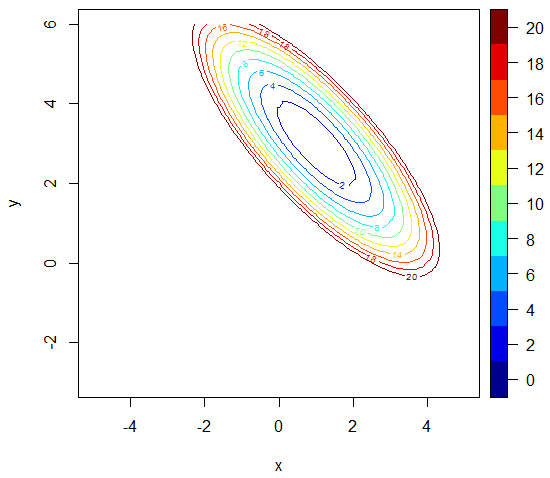
\includegraphics[scale=0.666]{q5}
\end{center}

O mínimo ocorre em $x^* = (1,3)$, $p(x^*) = 0$.

\singlespacing

\newpage

\begin{verbatim}
library('plot3D')
Mx1 <- -5
Mx2 <- 5
My1 <- -3
My2 <- 6
delta <- 0.1
x <- seq(Mx1, Mx2, delta)
y <- seq(My1, My2, delta)
M <- matrix(0,nrow=length(x),ncol=length(y))
for (i in 1:length(x))
  for (j in 1:length(y))
     M[i,j]<- (x[i] + 2*y[j] - 7)^2 + (2*x[i] + y[j] - 5)^2

min(M)
for (i in 1:length(x))
  for (j in 1:length(y))
    if (M[i,j] == min(M)) {
       print(x[i])
       print(y[j])
    }

contour2D(M,x,y,colkey = NULL,zlim=c(0,20)) 
\end{verbatim}

\vspace{6mm}

\large

\textbf{Questão 6}

\normalsize

\vspace{6mm}

\doublespacing

Faça o gráfico de contorno para a função $q(x_1, x_2) = 2(x_2 - x_1^2)^2 +(1 - x_1)^2$ na região $(-4 \le x_1 \le 4, -3 \le x_2 \le 6)$ e identifique o ponto ótimo.

\begin{center}
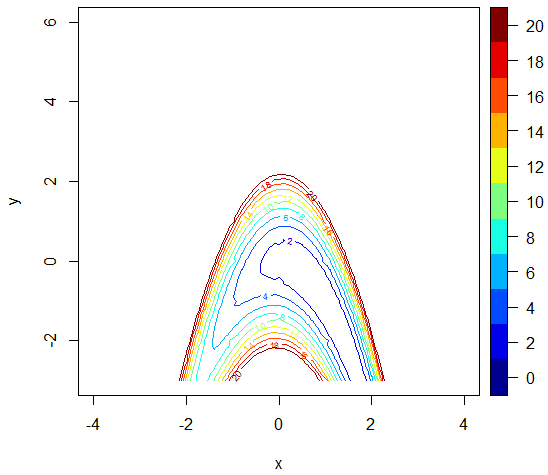
\includegraphics[scale=0.666]{q6}
\end{center}

O mínimo ocorre em $x^* = (1,-1)$, $q(x^*) = 0$.

Fontes abaixo.

\singlespacing

\newpage

\begin{verbatim}
Mx1 <- -4
Mx2 <- 4
My1 <- -3
My2 <- 6
delta <- 0.1
x <- seq(Mx1, Mx2, delta)
y <- seq(My1, My2, delta)
M <- matrix(0,nrow=length(x),ncol=length(y))
for (i in 1:length(x))
  for (j in 1:length(y))
     M[i,j]<- (2*y[j] + 2*x[i]^2)^2 + (1 - x[i])^2

min(M)
for (i in 1:length(x))
  for (j in 1:length(y))
    if (M[i,j] == min(M)) {
       print(x[i])
       print(y[j])
    }

contour2D(M,x,y,colkey = NULL,zlim=c(0,20)) 
\end{verbatim}

\vspace{6mm}

\large

\textbf{Questão 7}

\normalsize

\vspace{6mm}

\doublespacing

Realize duas iterações do Método de Newton para minimizar a função $h(x, y) = 100(y - x^2)^2 +(1 - x)^2$ com um $(x_0, y_0) = (-1.2, 1.0)$.

$\nabla h(x,y) = (-400x(y - x^2) - 2(1 - x), 200(y - x^2))$

$\nabla h(-1.2, 1.0) = (-215.6,-88)$

$H(x,y) = \begin{pmatrix} -400(y - 3x^2) + 2 & -400x  \\ -400x & 200 \end{pmatrix}$

$H(-1.2, 1.0) = \begin{pmatrix} 1330 & 480 \\ 480 & 200 \end{pmatrix} = H_1$

$(x_1, y_1) = (-1.2, 1.0) - H_1^{-1} \cdot (-215.6,-88) = (-1.175281, 1.380674)$

$\nabla h(-1.175281, 1.380674) = (-4.6378164,-0.1222068)$

$H(-1.175281, 1.380674) = \begin{pmatrix} 1107.2726 & 470.1124 \\ 470.1124 & 200 \end{pmatrix} = H_2$

$(x_2, y_2) = (-1.175281, 1.380674) - H_2^{-1} \cdot (-4.6378164,-0.1222068) = (0.7631149, -3.175034)$ ; $h(x_2, y_2) = 1411.845$.

Péssimo. Mas, continuando, o mínimo ocorre em $(x_3, y_3) = (0.7634297, 0.5828248)$ ; $h(x_3, y_3) = 0.05596552$.

\singlespacing

\newpage

\large

\textbf{Questão 8}

\normalsize

\vspace{6mm}

\doublespacing

Compare os gradientes da função $h(x, y)$ em $(x_0, y_0) = (0.5, 0.5)$ obtidos utilizando os seguintes métodos:

a) Resolução analítica:

$\nabla h(x,y) = (-400x(y - x^2) - 2(1 - x), 200(y - x^2))$

$v_1 = \nabla h(0.5, 0.5) = (-51,50) = (p_1, q_1)$

b) Método da diferença centrada:

Sejam $\Delta x = \Delta y = 0.0001$.

$p_2 = \cfrac{\partial h}{\partial x} = \cfrac{h(x + \Delta x,y) - h(x - \Delta x,y)}{2\Delta x} = \cfrac{h(0.5001,0.5) - h(0.4999,0.5)}{0.0001}$

$q_2 = \cfrac{\partial h}{\partial y} = \cfrac{h(x,y + \Delta y) - h(x,y - \Delta y)}{2\Delta y} = \cfrac{h(0.5,0.5001) - h(0.5,0.4999)}{0.0001}$

$v_2 = (p_2, q_2) = (-51,50)$.

c) Método da diferença progressiva:

$p_3 = \cfrac{\partial h}{\partial x} = \cfrac{h(x + \Delta x,y) - h(x,y)}{\Delta x} = \cfrac{h(0.5001,0.5) - h(0.5,0.5)}{0.0001}$

$q_3 = \cfrac{\partial h}{\partial y} = \cfrac{h(x,y + \Delta y) - h(x,y)}{\Delta y} = \cfrac{h(0.5,0.5001) - h(0.5,0.5)}{0.0001}$

$v_3 = (p_3, q_3) = (-50.9949, 50.0100)$.

d) Método da diferença regressiva:

$p_4 = \cfrac{\partial h}{\partial x} = \cfrac{h(x,y) - h(x - \Delta x,y)}{\Delta x} = \cfrac{h(0.5,0.5) - h(0.4999,0.5)}{0.0001}$

$q_4 = \cfrac{\partial h}{\partial y} = \cfrac{h(x,y) - h(x,y - \Delta y)}{\Delta y} = \cfrac{h(0.5,0.5) - h(0.5,0.4999)}{0.0001}$

$v_4 = (p_4, q_4) = (-51.0051, 49.9900)$.

e) Comparação:

$v_2 = v_1$ ; $p_3 > p_1$ ; $q_3 > q_1$ ; $p_4 < p_1$ ; $q_4 < q_1$.

$\vert p_3 - p_1 \vert = 0.0051 = \vert p_4 - p_1 \vert$ ; $\cfrac{0.0051}{51} = 0.01\%$ de erro.

$\vert q_3 - q_1 \vert = 0.01 = \vert q_4 - q_1 \vert$ ; $\cfrac{0.01}{50} = 0.02\%$ de erro.

\singlespacing

\newpage

\large

\textbf{Questão 9}

\normalsize

\vspace{6mm}

\doublespacing

Realize duas iterações do Método de Newton para minimizar a função $\varphi(x, y) = 2 x^2 + y^2$ com um $(x_0, y_0) = (1, 2)$.

$\nabla \varphi(x,y) = (4x, 2y)$

$\nabla \varphi(1, 2) = (4, 4)$

$H = \begin{pmatrix} 4 & 0 \\ 0 & 2 \end{pmatrix} \Rightarrow H^{-1} = \begin{pmatrix} 0.25 & 0 \\ 0 & 0.5 \end{pmatrix}$

$(x_1, y_1) = (1, 2) - \begin{pmatrix} 0.25 & 0 \\ 0 & 0.5 \end{pmatrix} \cdot (4, 4) = (0 , 0)$

$\nabla \varphi(0, 0) = (0, 0)$

O mínimo ocorre em $(x_2, y_2) = (0, 0) - \begin{pmatrix} 0.25 & 0 \\ 0 & 0.5 \end{pmatrix} \cdot (0, 0) = (0, 0)$ ; $\varphi(x_2, y_2) = 0$.

\singlespacing

\vspace{6mm}

\large

\textbf{Questão 10}

\normalsize

\vspace{6mm}

\doublespacing

Realize duas iterações do Método de Newton para minimizar a função $\psi(x, y, z) = x^2 + 3 y^2 + 6 z^2$ com um 

$(x_0, y_0, z_0) = (2, -1, 1)$.

$\nabla \psi(x,y,z) = (2x, 6y, 12z)$

$\nabla \psi(2, -1, 1) = (4, -6, 12)$

$H = \begin{pmatrix} 2 & 0 & 0 \\ 0 & 6 & 0 \\ 0 & 0 & 12 \end{pmatrix} \Rightarrow H^{-1} = \begin{pmatrix} 0.5 & 0 & 0 \\ 0 & 1/6 & 0 \\ 0 & 0 & 1/12 \end{pmatrix}$

$(x_1, y_1, z_1) = (2, -1, 1) - \begin{pmatrix} 0.5 & 0 & 0 \\ 0 & 1/6 & 0 \\ 0 & 0 & 1/12 \end{pmatrix} \cdot (4, -6, 12) = (0 , 0, 0)$

$\nabla \psi(0, 0, 0) = (0, 0, 0)$

O mínimo ocorre em $(x_2, y_2, z_2) = (0, 0, 0) - \begin{pmatrix} 0.5 & 0 & 0 \\ 0 & 1/6 & 0 \\ 0 & 0 & 1/12 \end{pmatrix} \cdot (0, 0, 0) = (0, 0, 0)$ ; $\psi(x_2, y_2, z_2) = 0$.

\singlespacing

\vspace{6mm}

Versão de 10/janeiro/2022\footnote{Fora da caridade não há salvação.} por Vinicius Claudino Ferraz.

\end{document}
